\documentclass[final]{beamer}
\usepackage[orientation=landscape,size=a0,scale=1.4]{beamerposter}
\usepackage[utf8]{inputenc}
\usepackage[T1]{fontenc}
\usepackage{times}
\usepackage{amsmath,amssymb}
\usepackage{graphicx}
\usepackage{booktabs}
\usepackage{tcolorbox}
\tcbuselibrary{skins,raster}

% Theme styling
\definecolor{bannerbg}{RGB}{245, 230, 220}
\definecolor{headerblue}{RGB}{18, 52, 86}
\definecolor{borderblue}{RGB}{100, 150, 190}
\setbeamercolor{background canvas}{bg=white}

\begin{document}
\begin{frame}[t]

% --- HEADER BANNER ---
\begin{tcolorbox}[colback=bannerbg, colframe=borderblue, width=\textwidth, arc=3mm, boxrule=1mm]
\begin{columns}[c]
    \begin{column}{0.12\textwidth}
        \centering
        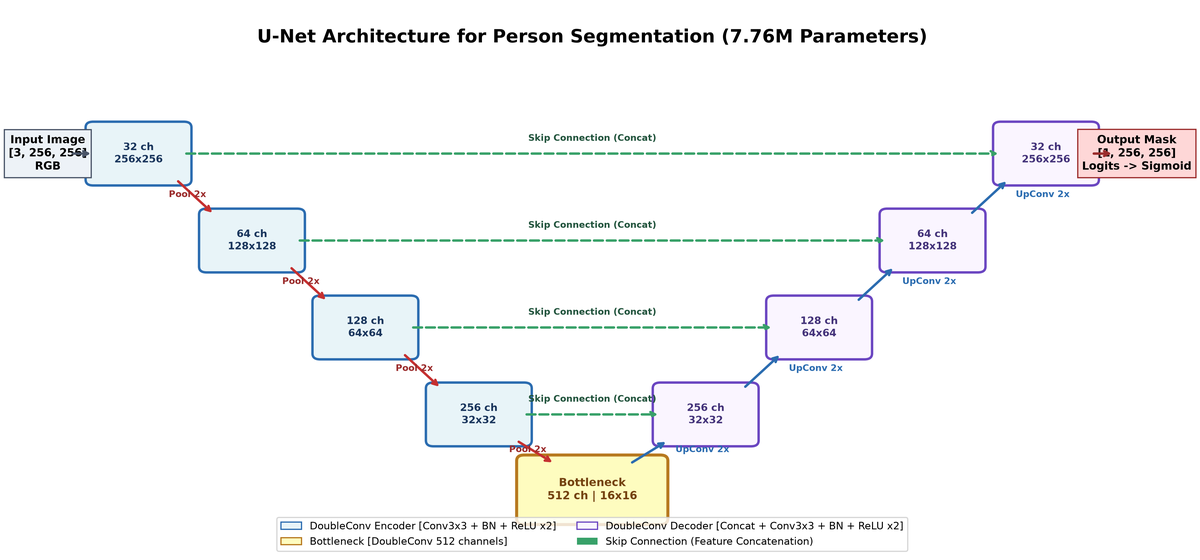
\includegraphics[height=5cm]{figures/unet_architecture.png}
    \end{column}
    \begin{column}{0.76\textwidth}
        \centering
        {\Huge\bfseries\color{headerblue} Deep Learning-Based Binary Person Segmentation Using Fully Convolutional U-Net \par}
        \vspace{0.4cm}
        {\LARGE\textbf{Mohith Chandra} \quad | \quad Department of Computer Science \quad | \quad Penn-Fudan Pedestrian Project \par}
    \end{column}
    \begin{column}{0.12\textwidth}
        \centering
        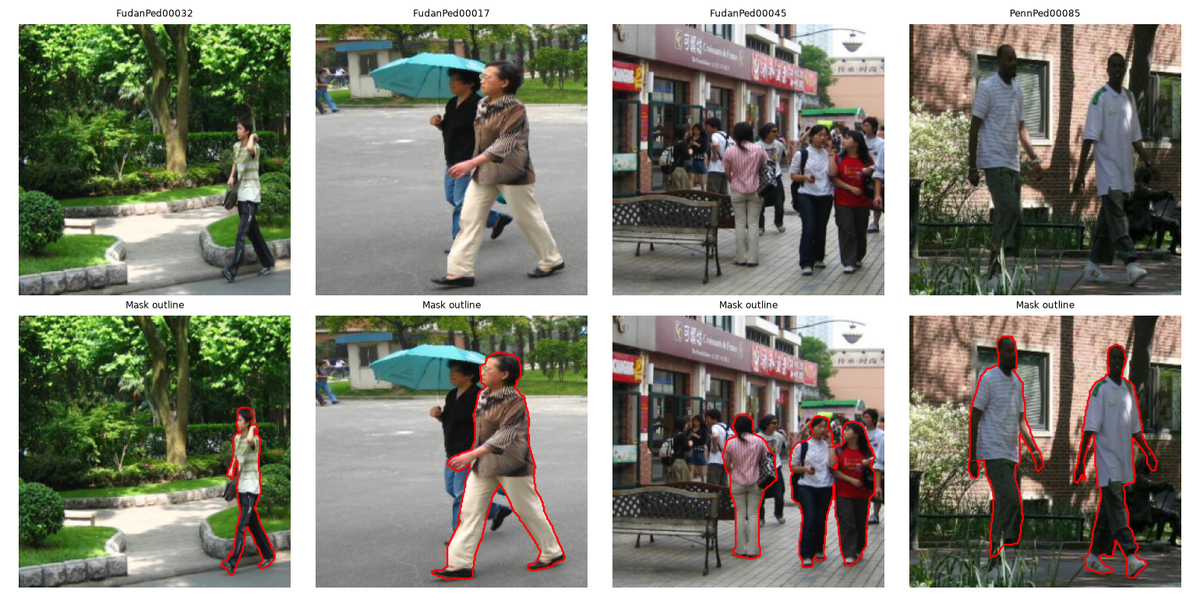
\includegraphics[height=5cm]{figures/pipeline_check.png}
    \end{column}
\end{columns}
\end{tcolorbox}

\vspace{0.6cm}

% --- 3-COLUMN CONTENT LAYOUT ---
\begin{columns}[t]

    % ==================== COLUMN 1 ====================
    \begin{column}{0.31\textwidth}
        
        \begin{tcolorbox}[colback=white, colframe=headerblue, title={\Large\bfseries Abstract}, arc=2mm, boxrule=0.8mm]
        {\large This project investigates end-to-end binary person segmentation on the Penn-Fudan dataset using an optimized U-Net trained from scratch. We systematically optimize data augmentation, learning rate, loss weight balancing, and model capacity. Our best model achieves \textbf{0.7739 Val IoU} and generalizes to \textbf{0.7483 Global Test IoU} and \textbf{0.7616 Mean Per-Image IoU} on 27 unseen test scenes.}
        \end{tcolorbox}

        \vspace{0.4cm}

        \begin{tcolorbox}[colback=white, colframe=headerblue, title={\Large\bfseries Introduction \& Problem Statement}, arc=2mm, boxrule=0.8mm]
        {\large
        \begin{itemize}
            \item Pedestrian segmentation is critical for autonomous navigation and surveillance.
            \item Real-world scenes present severe scale variation, human pose deformability, occlusions, and foreground/background class imbalance ($23.2\%$ vs $76.8\%$).
            \item Small-sample training ($118$ images) requires robust regularization to prevent empirical memorization.
        \end{itemize}}
        \end{tcolorbox}

        \vspace{0.4cm}

        \begin{tcolorbox}[colback=white, colframe=headerblue, title={\Large\bfseries Key Contributions}, arc=2mm, boxrule=0.8mm]
        {\large
        \begin{itemize}
            \item \textbf{From-Scratch U-Net:} Fully modular 4-stage encoder-decoder backbone in PyTorch with skip connections ($7.76$M parameters).
            \item \textbf{Synchronized Augmentation:} Bilateral flip ($p=0.5$) and scale zoom ($0.9$--$1.1\times$), delivering $+2.53\%$ relative IoU improvement.
            \item \textbf{Asymmetric Hybrid Loss:} Balanced $\alpha \mathcal{L}_{\text{BCE}} + \beta \mathcal{L}_{\text{Dice}}$ ($1.5/0.5$) prioritizing boundary precision over background clutter.
            \item \textbf{Noise Discovery:} Identified ground-truth label omissions on background pedestrians in the test split.
        \end{itemize}}
        \end{tcolorbox}

    \end{column}

    % ==================== COLUMN 2 ====================
    \begin{column}{0.35\textwidth}
        
        \begin{tcolorbox}[colback=white, colframe=headerblue, title={\Large\bfseries Proposed U-Net Architecture \& Methodology}, arc=2mm, boxrule=0.8mm]
        \centering
        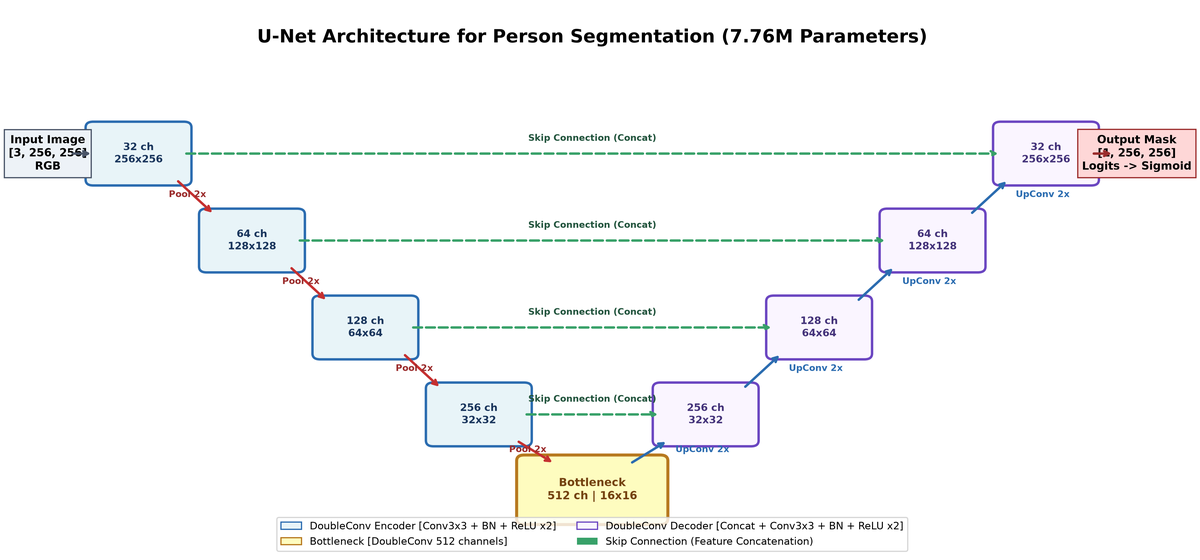
\includegraphics[width=0.98\linewidth]{figures/unet_architecture.png}
        \vspace{0.2cm}
        {\small\textbf{Figure 1:} Fully Convolutional U-Net topology with 4 contracting and 4 expanding stages.}
        \end{tcolorbox}

        \vspace{0.4cm}

        \begin{tcolorbox}[colback=white, colframe=headerblue, title={\Large\bfseries Optimization Algorithm \& Training Pipeline}, arc=2mm, boxrule=0.8mm]
        {\small
        \textbf{Algorithm 1: End-to-End Hybrid U-Net Optimization}
        \begin{enumerate}
            \item Split dataset ($170$ images) into $118$ train, $25$ val, and $27$ test (seed 42).
            \item Initialize U-Net ($C=32$, $7.76$M params) with Kaiming normal.
            \item For each epoch:
            \begin{itemize}
                \item Forward batch with synchronized flip and scale zoom.
                \item Compute $\mathcal{L} = 1.5 \mathcal{L}_{\text{BCE}} + 0.5 \mathcal{L}_{\text{Dice}}$ ($\text{smooth}=1.0$).
                \item Backpropagate using Adam ($\eta=5\times 10^{-4}$).
            \end{itemize}
            \item Evaluate on untouched validation set; monitor validation IoU.
            \item Step ReduceLROnPlateau; checkpoint best model; early stop at patience 20.
        \end{enumerate}}
        \end{tcolorbox}

    \end{column}

    % ==================== COLUMN 3 ====================
    \begin{column}{0.31\textwidth}
        
        \begin{tcolorbox}[colback=white, colframe=headerblue, title={\Large\bfseries Experimental Results \& Discussion}, arc=2mm, boxrule=0.8mm]
        \centering
        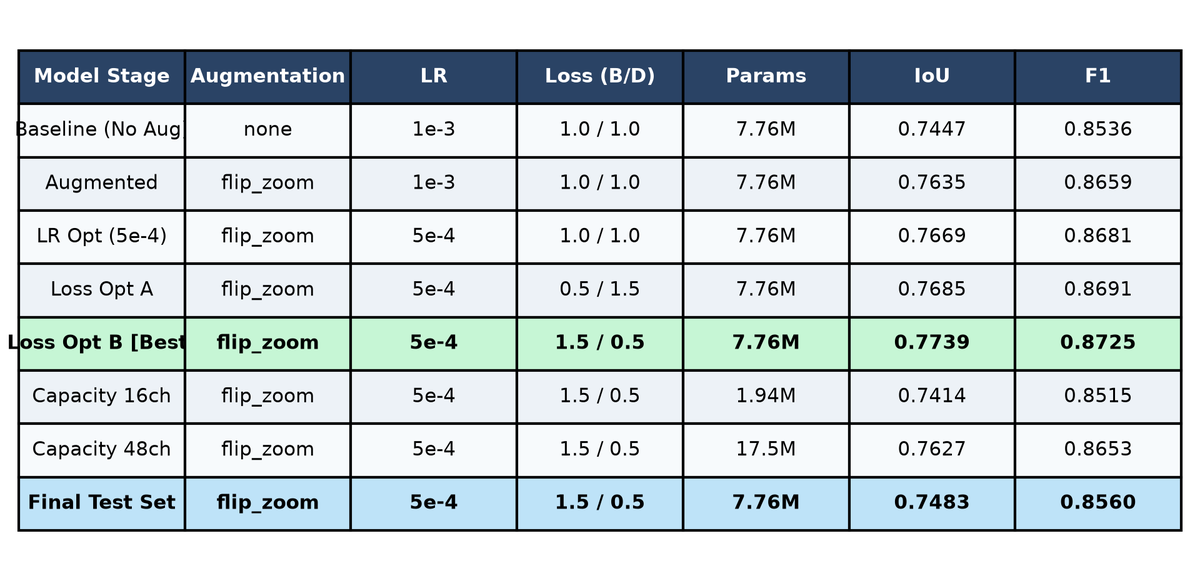
\includegraphics[width=0.98\linewidth]{figures/table1_poster.png}
        \vspace{0.2cm}
        {\small\textbf{Table 1:} Cross-phase progression on validation and unseen test sets.}
        
        \vspace{0.3cm}
        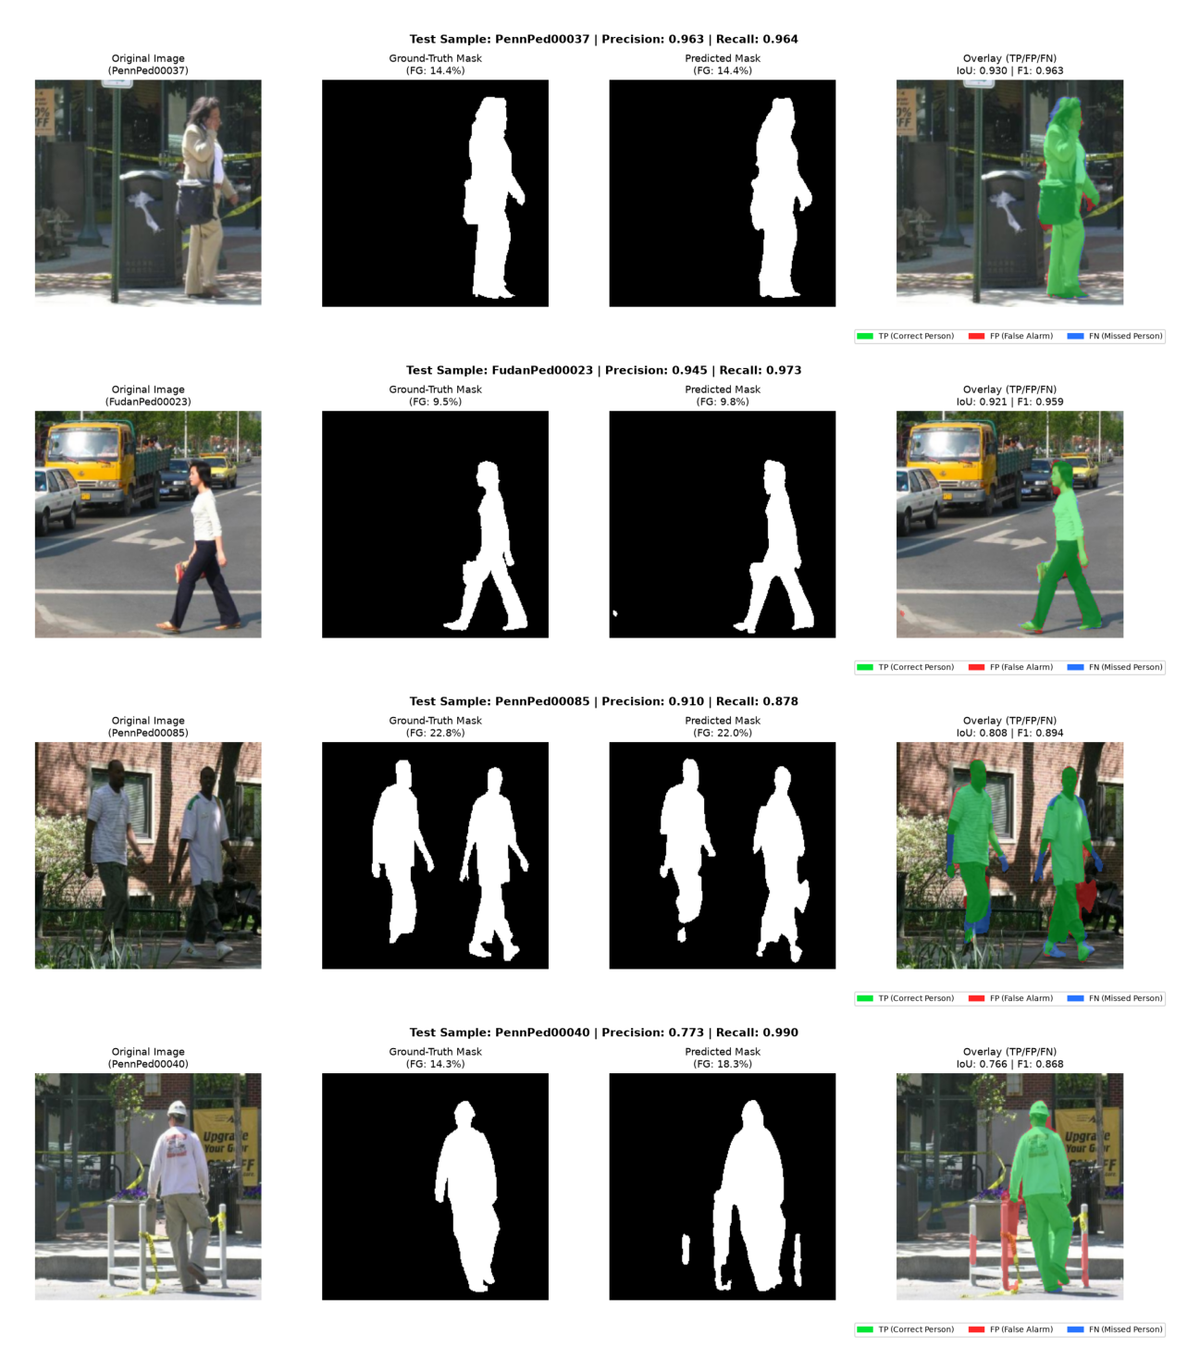
\includegraphics[width=0.98\linewidth]{figures/predictions_poster.png}
        \vspace{0.2cm}
        {\small\textbf{Figure 2:} Visual test predictions showing overlay alignment.}
        \end{tcolorbox}

        \vspace{0.4cm}

        \begin{tcolorbox}[colback=white, colframe=headerblue, title={\Large\bfseries Conclusion}, arc=2mm, boxrule=0.8mm]
        {\large An optimized from-scratch U-Net achieves \textbf{0.7483 Global Test IoU} and \textbf{0.8936 Recall}. Systematic loss reweighting and synchronized augmentation effectively conquer sample scarcity.}
        \end{tcolorbox}

        \vspace{0.2cm}

        \begin{tcolorbox}[colback=white, colframe=headerblue, title={\small\bfseries Key References}, arc=1mm, boxrule=0.5mm]
        {\tiny
        [1] Ronneberger et al. U-Net: Convolutional Networks for Biomedical Image Segmentation. MICCAI, 2015.\\
        [2] Wang et al. Object Detection Combining Recognition and Segmentation. IEEE TPAMI, 2008.\\
        [3] Milletari et al. V-Net: Fully Convolutional Networks for Volumetric Medical Image Segmentation. 3DV, 2016.}
        \end{tcolorbox}

    \end{column}

\end{columns}

\end{frame}
\end{document}

